% -*- Mode:TeX -*-

%% IMPORTANT: The official thesis specifications are available at:
%%            http://libraries.mit.edu/archives/thesis-specs/
%%
%%            Please verify your thesis' formatting and copyright
%%            assignment before submission.  If you notice any
%%            discrepancies between these templates and the
%%            MIT Libraries' specs, please let us know
%%            by e-mailing thesis@mit.edu

%% The documentclass options along with the pagestyle can be used to generate
%% a technical report, a draft copy, or a regular thesis.  You may need to
%% re-specify the pagestyle after you \include  cover.tex.  For more
%% information, see the first few lines of mitthesis.cls.

%\documentclass[12pt,vi,twoside]{mitthesis}
%%
%%  If you want your thesis copyright to you instead of MIT, use the
%%  ``vi'' option, as above.
%%
%\documentclass[12pt,twoside,leftblank]{mitthesis}
%%
%% If you want blank pages before new chapters to be labelled ``This
%% Page Intentionally Left Blank'', use the ``leftblank'' option, as
%% above.

\documentclass[11pt,twoside]{mitthesis}
\usepackage{lgrind}
%% These have been added at the request of the MIT Libraries, because
%% some PDF conversions mess up the ligatures.  -LB, 1/22/2014
\usepackage{setspace}
\usepackage{cmap}
\usepackage{graphicx}
\usepackage[utf8]{inputenc}
\usepackage[T1]{fontenc}
\usepackage{lmodern}
\pagestyle{plain}
\onehalfspace

%% This bit allows you to either specify only the files which you wish to
%% process, or `all' to process all files which you \include.
%% Krishna Sethuraman (1990).

%\typein [\files]{Enter file names to process, (chap1,chap2 ...), or `all' to
%process all files:}

%\def\all{all}

%\ifx\files\all \typeout{Including all files.} \else \typeout{Including only \files.} \includeonly{\files} \fi

\begin{document}

% -*-latex-*-
%
% For questions, comments, concerns or complaints:
% thesis@mit.edu
%
%
% $Log: cover.tex,v $
% Revision 1.8  2008/05/13 15:02:15  jdreed
% Degree month is June, not May.  Added note about prevdegrees.
% Arthur Smith's title updated
%
% Revision 1.7  2001/02/08 18:53:16  boojum
% changed some \newpages to \cleardoublepages
%
% Revision 1.6  1999/10/21 14:49:31  boojum
% changed comment referring to documentstyle
%
% Revision 1.5  1999/10/21 14:39:04  boojum
% *** empty log message ***
%
% Revision 1.4  1997/04/18  17:54:10  othomas
% added page numbers on abstract and cover, and made 1 abstract
% page the default rather than 2.  (anne hunter tells me this
% is the new institute standard.)
%
% Revision 1.4  1997/04/18  17:54:10  othomas
% added page numbers on abstract and cover, and made 1 abstract
% page the default rather than 2.  (anne hunter tells me this
% is the new institute standard.)
%
% Revision 1.3  93/05/17  17:06:29  starflt
% Added acknowledgements section (suggested by tompalka)
%
% Revision 1.2  92/04/22  13:13:13  epeisach
% Fixes for 1991 course 6 requirements
% Phrase "and to grant others the right to do so" has been added to
% permission clause
% Second copy of abstract is not counted as separate pages so numbering works
% out
%
% Revision 1.1  92/04/22  13:08:20  epeisach

% NOTE:
% These templates make an effort to conform to the MIT Thesis specifications,
% however the specifications can change.  We recommend that you verify the
% layout of your title page with your thesis advisor and/or the MIT
% Libraries before printing your final copy.
\title{Improving house security using an IoT infrastructure}

\author{Mirko Morandi}
% If you wish to list your previous degrees on the cover page, use the
% previous degrees command:
%       \prevdegrees{A.A., Harvard University (1985)}
% You can use the \\ command to list multiple previous degrees
%       \prevdegrees{B.S., University of California (1978) \\
%                    S.M., Massachusetts Institute of Technology (1981)}
\department{Department of Computer Science}

% If the thesis is for two degrees simultaneously, list them both
% separated by \and like this:
% \degree{Doctor of Philosophy \and Master of Science}
\degree{Master Degree in Computer Science}

% As of the 2007-08 academic year, valid degree months are September,
% February, or June.  The default is June.
\degreemonth{June}
\degreeyear{2016}
\thesisdate{June 18, 2016}

%% By default, the thesis will be copyrighted to MIT.  If you need to copyright
%% the thesis to yourself, just specify the `vi' documentclass option.  If for
%% some reason you want to exactly specify the copyright notice text, you can
%% use the \copyrightnoticetext command.
%\copyrightnoticetext{\copyright IBM, 1990.  Do not open till Xmas.}

% If there is more than one supervisor, use the \supervisor command
% once for each.
\supervisor{Kitlei Ròbert}{ELTE Supervisor}
\supervisor{Marchese Maurizio}{Trento Supervisor}
\supervisor{László Szilágyi}{Industrial Supervisor}
% This is the department committee chairman, not the thesis committee
% chairman.  You should replace this with your Department's Committee
% Chairman.
%\chairman{Arthur C. Smith}{Chairman, Department Committee on Graduate Theses}

% Make the titlepage based on the above information.  If you need
% something special and can't use the standard form, you can specify
% the exact text of the titlepage yourself.  Put it in a titlepage
% environment and leave blank lines where you want vertical space.
% The spaces will be adjusted to fill the entire page.  The dotted
% lines for the signatures are made with the \signature command.
\maketitle

% The abstractpage environment sets up everything on the page except
% the text itself.  The title and other header material are put at the
% top of the page, and the supervisors are listed at the bottom.  A
% new page is begun both before and after.  Of course, an abstract may
% be more than one page itself.  If you need more control over the
% format of the page, you can use the abstract environment, which puts
% the word "Abstract" at the beginning and single spaces its text.

%% You can either \input (*not* \include) your abstract file, or you can put
%% the text of the abstract directly between the \begin{abstractpage} and
%% \end{abstractpage} commands.

% First copy: start a new page, and save the page number.
\newpage
% Uncomment the next line if you do NOT want a page number on your
% abstract and acknowledgments pages.
%\pagestyle{empty}
\setcounter{savepage}{\thepage}
\begin{abstractpage}
% $Log: abstract.tex,v $
% Revision 1.1  93/05/14  14:56:25  starflt
% Initial revision
%
% Revision 1.1  90/05/04  10:41:01  lwvanels
% Initial revision
%
%
%% The text of your abstract and nothing else (other than comments) goes here.
%% It will be single-spaced and the rest of the text that is supposed to go on
%% the abstract page will be generated by the abstractpage environment.  This
%% file should be \input (not \include 'd) from cover.tex.

The recent increase of power of computation combined to the decrease of power
consumption of devices led to an explosion of smart devices for all the possible
purposes, and it's called the \textit{\textbf{Internet of Things}}.\\
The IoT includes all devices that has an interface to the real world
and are connected to the Internet, such as: \textit{Smart Fridges, Smart TVs, Thermostats,
Alarms, Cameras and etc}. These devices were born to simplify normal people's life,
let's take the smart fridge as example: it will alert you when the food you have in the
fridge is going to expire, the thermostat will try to save money applying smart
strategies for heat consumption. One of the most important application of IoT
to people's life is \textit{House Security}: exploiting the IoT concept to improve the house
security with smart sensors like cameras, leap motion sensors and microphones.
House Security has to be of concern, because house invasion is an always trending
crime. However these systems are not always perfect and the most common problem are
false positives, for the which there is an active branch of research focused on.\\
The raise of devices connected introduced another problem: heterogeneity between
IoT devices. As the popularity of smart devices increased more and more companies
started producing their own different ecosystems. Communication between different
ecosystems is another research topic which will analyzed in this document.

\end{abstractpage}

% Additional copy: start a new page, and reset the page number.  This way,
% the second copy of the abstract is not counted as separate pages.
% Uncomment the next 6 lines if you need two copies of the abstract
% page.
% \setcounter{page}{\thesavepage}
% \begin{abstractpage}
% % $Log: abstract.tex,v $
% Revision 1.1  93/05/14  14:56:25  starflt
% Initial revision
%
% Revision 1.1  90/05/04  10:41:01  lwvanels
% Initial revision
%
%
%% The text of your abstract and nothing else (other than comments) goes here.
%% It will be single-spaced and the rest of the text that is supposed to go on
%% the abstract page will be generated by the abstractpage environment.  This
%% file should be \input (not \include 'd) from cover.tex.

The recent increase of power of computation combined to the decrease of power
consumption of devices led to an explosion of smart devices for all the possible
purposes, and it's called the \textit{\textbf{Internet of Things}}.\\
The IoT includes all devices that has an interface to the real world
and are connected to the Internet, such as: \textit{Smart Fridges, Smart TVs, Thermostats,
Alarms, Cameras and etc}. These devices were born to simplify normal people's life,
let's take the smart fridge as example: it will alert you when the food you have in the
fridge is going to expire, the thermostat will try to save money applying smart
strategies for heat consumption. One of the most important application of IoT
to people's life is \textit{House Security}: exploiting the IoT concept to improve the house
security with smart sensors like cameras, leap motion sensors and microphones.
House Security has to be of concern, because house invasion is an always trending
crime. However these systems are not always perfect and the most common problem are
false positives, for the which there is an active branch of research focused on.\\
The raise of devices connected introduced another problem: heterogeneity between
IoT devices. As the popularity of smart devices increased more and more companies
started producing their own different ecosystems. Communication between different
ecosystems is another research topic which will analyzed in this document.

% \end{abstractpage}

\newpage

\section*{Acknowledgments}

This is the acknowledgements section.  You should replace this with your
own acknowledgements.

%%%%%%%%%%%%%%%%%%%%%%%%%%%%%%%%%%%%%%%%%%%%%%%%%%%%%%%%%%%%%%%%%%%%%%
% -*-latex-*-

%%% This file is for producing a Doctoral Thesis proposal.  It should be fairly
%% self-explanatory.  

\documentclass{article}
\begin{document}

\bibliographystyle{plain}
\pagestyle{empty}
\markboth{{\sc thesis proposal}}{{\sc thesis proposal}}
\def\title{Parallel Processor Architecture}
\def\author{Peter Nuth}
\def\addrone{305 Memorial Drive, 606C}
\def\addrtwo{Cambridge, MA  02139}

\def\degree{Doctor of Philosophy}
%% Added \deptname for PhD proposals in other fields.
%% Krishna Sethuraman (1990)
\def\deptname{Electrical Engineering \\ and Computer Science}
\def\laboratory{Artificial Intelligence Laboratory}

\def\submissiondate{\today}
\def\completiondate{September 1990}

\def\supervisor{Professor William J. Dally}
\def\supertitleone{Associate Professor of Electrical Engineering}
\def\supertitletwo{and Computer Science}

\def\readerone{Professor Arvind}
\def\readeronetitleone{Professor of Electrical Engineering}
\def\readeronetitletwo{and Computer Science}

\def\readertwo{Professor Thomas Knight}
\def\readertwotitleone{Assistant Professor of Electrical Engineering}
\def\readertwotitletwo{and Computer Science}

\def\readerthree{Professor William J. Dally}
\def\readerthreetitleone{Associate Professor of Electrical Engineering}
\def\readerthreetitletwo{and Computer Science}


\def\abstract{
The proposed research
is a study of processor architecture for 
large scale parallel computer systems.
The thesis introduces mechanisms
for fast context switching, 
synchronization between tasks,
and run-time binding of 
variable names to processor memory.
Various design tradeoffs are evaluated 
through simulation of a processor running a typical load.
This work contains
estimates of
the speed and complexity of the different 
alternatives as implemented in  VLSI.
}

%%%%%%%%%%%%%%%%%%%%%%%%%%%%%%%%%%%%%%%%%%%%%%%%%%%%%%%%%%%%%%%%%%%%%%%%%%%%
%%%%%%%%%% You Should Not Need To Modify Anything Below Here %%%%%%%%%%%%%%%
%%%%%%%%%%%%%%%%%%%%%%%%%%%%%%%%%%%%%%%%%%%%%%%%%%%%%%%%%%%%%%%%%%%%%%%%%%%%

%%%%%%%%%%%%%%%%%%%%%%%%%%%%%%%%%
%%% Cover Page - Author signs %%%
%%%%%%%%%%%%%%%%%%%%%%%%%%%%%%%%%

\begin{center}
{\Large \bf 
   Massachusetts Institute of Technology
\\ Department of \deptname \\}
\vspace{.25in}
{\Large \bf
   Proposal for Thesis Research in Partial Fulfillment
\\ of the Requirements for the Degree of
\\ \degree \\}
\end{center}

\vspace{.5in}

\def\sig{{\small \sc (Signature of Author)}}

\begin{tabular}{rlc}
   {\small \sc Title:}                       & \multicolumn{2}{l}{\title}
\\ {\small \sc Submitted by:}
                            & \author  & \\
                            & \addrone & \\
                            & \addrtwo & \\ \cline{3-3}
			    &	       & \makebox[2in][c]{\sig}
\\ {\small \sc Date of Submission:}          & \multicolumn{2}{l}{\submissiondate}
\\ {\small \sc Expected Date of Completion:} & \multicolumn{2}{l}{\completiondate}
\\ {\small \sc Laboratory:}                  & \multicolumn{2}{l}{\laboratory}
\end{tabular}


\vspace{.75in}
{\bf \sc Brief Statement of the Problem:}

\abstract

         %%%%%%%%%%%%%%%%%%%%%%%%%%%%%
\newpage %%% Supervision Agreement %%%
         %%%%%%%%%%%%%%%%%%%%%%%%%%%%%

\begin{flushright}
   Massachusetts Institute of Technology
\\ Department of \deptname
\\ Cambridge, Massachusetts 02139
\end{flushright}

\underline{\bf Doctoral Thesis Supervision Agreement}

\vspace{.25in}
\begin{tabular}{rl}
   {\small \sc To:}   & Department Graduate Committee
\\ {\small \sc From:} & \supervisor
\end{tabular}

\vspace{.25in}
The program outlined in the proposal:

\vspace{.25in}
\begin{tabular}{rl}
   {\small \sc Title:}  & \title
\\ {\small \sc Author:} & \author
\\ {\small \sc Date:}   & \submissiondate
\end{tabular}

\vspace{.25in}
is adequate for a Doctoral thesis.
I believe that appropriate readers for this thesis would be:

\vspace{.25in}
\begin{tabular}{rl}
   {\small \sc Reader 1:} & \readerone
\\ {\small \sc Reader 2:} & \readertwo
%\\ {\small \sc Reader 3:} & \readerthree
\end{tabular}

\vspace{.25in}
Facilities and support for the research outlined in the proposal are available.
I am willing to supervise the thesis and evaluate the thesis report.

\vspace{.25in}
\begin{tabular}{crc}
  \hspace{2in} & {\sc Signed:} & \\ \cline{3-3}
               &               & {\small \sc \supertitleone} \\
               &               & {\small \sc \supertitletwo} \\
               &               &                             \\
               & {\sc Date:}   & \\ \cline{3-3}
\end{tabular}

\vspace{0in plus 1fill}

Comments: \\
\begin{tabular}{c}
  \hspace{6.25in} \\
  \mbox{} \\ \cline{1-1} \mbox{} \\
  \mbox{} \\ \cline{1-1} \mbox{} \\
  \mbox{} \\ \cline{1-1} \mbox{} \\
%  \mbox{} \\ \cline{1-1} \mbox{} \\
%  \mbox{} \\ \cline{1-1} \mbox{} \\
%  \mbox{} \\ \cline{1-1} \mbox{} \\
\end{tabular}

          %%%%%%%%%%%%%%%%%%%%%%%%%%
\newpage  %%% Reader I Agreement %%%
          %%%%%%%%%%%%%%%%%%%%%%%%%%

\begin{flushright}
   Massachusetts Institute of Technology
\\ Department of \deptname
\\ Cambridge, Massachusetts 02139
\end{flushright}

\underline{\bf Doctoral Thesis Reader Agreement}

\vspace{.25in}
\begin{tabular}{rl}
   {\small \sc To:}   & Department Graduate Committee
\\ {\small \sc From:} & \readerone
\end{tabular}

\vspace{.25in}
The program outlined in the proposal:

\vspace{.25in}
\begin{tabular}{rl}
   {\small \sc Title:}          & \title
\\ {\small \sc Author:}         & \author
\\ {\small \sc Date:}           & \submissiondate
\\ {\small \sc Supervisor:}     & \supervisor
\\ {\small \sc Other Reader:}   & \readertwo
%\\ {\small \sc Other Reader:}   & \readerthree
\end{tabular}

\vspace{.25in}
is adequate for a Doctoral thesis.
I am willing to aid in guiding the research
and in evaluating the thesis report as a reader.

\vspace{.25in}
\begin{tabular}{crc}
  \hspace{2in} & {\sc Signed:} & \\ \cline{3-3}
               &               & {\small \sc \readeronetitleone} \\
               &               & {\small \sc \readeronetitletwo} \\
               &               &                                 \\
               & {\sc Date:}   & \\ \cline{3-3}
\end{tabular}

\vspace{0in plus 1fill}

Comments: \\
\begin{tabular}{c}
  \hspace{6.25in} \\
  \mbox{} \\ \cline{1-1} \mbox{} \\
  \mbox{} \\ \cline{1-1} \mbox{} \\
  \mbox{} \\ \cline{1-1} \mbox{} \\
  \mbox{} \\ \cline{1-1} \mbox{} \\
  \mbox{} \\ \cline{1-1} \mbox{} \\
  \mbox{} \\ \cline{1-1} \mbox{} \\
\end{tabular}


          %%%%%%%%%%%%%%%%%%%%%%%%%%%
\newpage  %%% Reader II Agreement %%%
          %%%%%%%%%%%%%%%%%%%%%%%%%%%


\begin{flushright}
   Massachusetts Institute of Technology
\\ Department of \deptname
\\ Cambridge, Massachusetts 02139
\end{flushright}

\underline{\bf Doctoral Thesis Reader Agreement}

\vspace{.25in}
\begin{tabular}{rl}
   {\small \sc To:}   & Department Graduate Committee
\\ {\small \sc From:} & \readertwo
\end{tabular}

\vspace{.25in}
The program outlined in the proposal:

\vspace{.25in}
\begin{tabular}{rl}
   {\small \sc Title:}          & \title
\\ {\small \sc Author:}         & \author
\\ {\small \sc Date:}           & \submissiondate
\\ {\small \sc Supervisor:}     & \supervisor
\\ {\small \sc Other Reader:}   & \readerone
%\\ {\small \sc Other Reader:}   & \readerthree
\end{tabular}

\vspace{.25in}
is adequate for a Doctoral thesis.
I am willing to aid in guiding the research
and in evaluating the thesis report as a reader.

\vspace{.25in}
\begin{tabular}{crc}
  \hspace{2in} & {\sc Signed:} & \\ \cline{3-3}
               &               & {\small \sc \readertwotitleone} \\
               &               & {\small \sc \readertwotitletwo} \\
               &               &                                 \\
               & {\sc Date:}   & \\ \cline{3-3}
\end{tabular}

\vspace{0in plus 1fill}

Comments: \\
\begin{tabular}{c}
  \hspace{6.25in} \\
  \mbox{} \\ \cline{1-1} \mbox{} \\
  \mbox{} \\ \cline{1-1} \mbox{} \\
  \mbox{} \\ \cline{1-1} \mbox{} \\
  \mbox{} \\ \cline{1-1} \mbox{} \\
  \mbox{} \\ \cline{1-1} \mbox{} \\
  \mbox{} \\ \cline{1-1} \mbox{} \\
\end{tabular}
\newpage
          %%%%%%%%%%%%%%%%%%%%%%%%%%%
\newpage  %%% Reader III Agreement %%%
          %%%%%%%%%%%%%%%%%%%%%%%%%%%


\begin{flushright}
   Massachusetts Institute of Technology
\\ Department of \deptname
\\ Cambridge, Massachusetts 02139
\end{flushright}

\underline{\bf Doctoral Thesis Reader Agreement}

\vspace{.25in}
\begin{tabular}{rl}
   {\small \sc To:}   & Department Graduate Committee
\\ {\small \sc From:} & \readerthree
\end{tabular}

\vspace{.25in}
The program outlined in the proposal:

\vspace{.25in}
\begin{tabular}{rl}
   {\small \sc Title:}          & \title
\\ {\small \sc Author:}         & \author
\\ {\small \sc Date:}           & \submissiondate
\\ {\small \sc Supervisor:}     & \supervisor
\\ {\small \sc Other Reader:}   & \readerone
\\ {\small \sc Other Reader:}   & \readertwo
\end{tabular}

\vspace{.25in}
is adequate for a Doctoral thesis.
I am willing to aid in guiding the research
and in evaluating the thesis report as a reader.

\vspace{.25in}
\begin{tabular}{crc}
  \hspace{2in} & {\sc Signed:} & \\ \cline{3-3}
               &               & {\small \sc \readerthreetitleone} \\
               &               & {\small \sc \readerthreetitletwo} \\
               &               &                                 \\
               & {\sc Date:}   & \\ \cline{3-3}
\end{tabular}

\vspace{0in plus 1fill}

Comments: \\
\begin{tabular}{c}
  \hspace{6.25in} \\
  \mbox{} \\ \cline{1-1} \mbox{} \\
  \mbox{} \\ \cline{1-1} \mbox{} \\
  \mbox{} \\ \cline{1-1} \mbox{} \\
  \mbox{} \\ \cline{1-1} \mbox{} \\
  \mbox{} \\ \cline{1-1} \mbox{} \\
  \mbox{} \\ \cline{1-1} \mbox{} \\
\end{tabular}
\newpage

\end{document}






% Some departments (e.g. 5) require an additional signature page.  See
% signature.tex for more information and uncomment the following line if
% applicable.
% % -*- Mode:TeX -*-
%
% Some departments (e.g. Chemistry) require an additional cover page
% with signatures of the thesis committee.  Please check with your
% thesis advisor or other appropriate person to determine if such a 
% page is required for your thesis.  
%
% If you choose not to use the "titlepage" environment, a \newpage
% commands, and several \vspace{\fill} commands may be necessary to
% achieve the required spacing.  The \signature command is defined in
% the "mitthesis" class
%
% The following sample appears courtesy of Ben Kaduk <kaduk@mit.edu> and
% was used in his June 2012 doctoral thesis in Chemistry. 

\begin{titlepage}
\begin{large}
This doctoral thesis has been examined by a Committee of the Department
of Chemistry as follows:

\signature{Professor Jianshu Cao}{Chairman, Thesis Committee \\
   Professor of Chemistry}

\signature{Professor Troy Van Voorhis}{Thesis Supervisor \\
   Associate Professor of Chemistry}

\signature{Professor Robert W. Field}{Member, Thesis Committee \\
   Haslam and Dewey Professor of Chemistry}
\end{large}
\end{titlepage}


\pagestyle{plain}
  % -*- Mode:TeX -*-
%% This file simply contains the commands that actually generate the table of
%% contents and lists of figures and tables.  You can omit any or all of
%% these files by simply taking out the appropriate command.  For more
%% information on these files, see appendix C.3.3 of the LaTeX manual. 
\tableofcontents
\newpage
\listoffigures
\newpage
\listoftables


%% This is an example first chapter.  You should put chapter/appendix that you
%% write into a separate file, and add a line \include{yourfilename} to
%% main.tex, where `yourfilename.tex' is the name of the chapter/appendix file.
%% You can process specific files by typing their names in at the
%% \files=
%% prompt when you run the file main.tex through LaTeX.
\chapter{Introduction}

IoT surveillance systems has been proved to be effective during the time,
catching the burglar committing the crime and helping the authorities to
catch him[1]. Nonetheless these systems are not yet perfect, and during
this paper we will investigate on some optimizations with respect to
the \textit{integration} with other ecosystems and the \textit{reduction}
of false positives.\\
Here follows the main structure of the document:\\

Chapter two introduces the technologies used in our scenario, with a brief
introduction on the techniques adopted to face the various problems.

Chapter three illustrates the main architecture of the optimizations proposed
during the document and the motivation behind them.

Chapter four shows the implementation of our use case with the optimizations
we have described formerly.

Chapter five is an extensive analysis of the results obtained during the whole
analysis of the scenario.

\section{Motivations}

The idea behind our research in this field is to improve the existing solution
with an innovative and different approach. Nowdays there are many standalone
solutions for IoT surveillance, which acts separately from all the other
components in the house. We address this isolation, trying to create
a system capable of interconnecting with other existing components in the house.
There are currently 4 billion of connected devices [2] as 2016, and the forecasts
says they will be 13.5b in 2020. This means a growth in the heterogenity of companies
and products, which makes a must the interopability between devices from different
producers.\\
Most of the common Smart devices are built to work appositely with their own application,
without any external support which leads to a loose coupling between devices.

%%[TODO] add stuff here, lacking of inspiration now

\section{Description of scenario}\label{ch1:opts}

During this document we will refer to a use case scenario related
to house security. In this scenario we will have a small house with different
floors, each floor having a leap motion sensor to detect any movement and a camera
recording.
\subsection{M2M: Machine to Machine}

Most of common smart sensors, in order to be \textit{smart} they need
to provide a form of connectivity: let it be BLE (Bluetooth Low Energy),
Wi-Fi or R-FID. \textit{M2M} is treanding with the raising of IoT,
requiring a higher number of devices to be interconnected without
any human interaction. Different devices means different protocols,
which introduces difficulties in the communications between each other.
The typical approach is to define a set of translators which
are able to deal with both sides, also called \textit{Gateways}.
Gateways are high-level objects that knows the various protocols
needed to communicate and provide these knowledge as a service to
whom has the necessity to access the functionalities provided by the
device. \\
In our architecture each gateway is a device exposing a service using
a \textbf{RESTful} architecture, for a better simplicity of use.

\subsection{Microservices and IoT}
\label{sub:microservicesiot}

The Microservice architecture is an innovative modelling pattern that aims
to solve a well defined class of problems: scaling.
The idea behind microservices is to split the architecture on different machines
usually communicating through a RESTful interface.
This pattern is similar to the \textit{microkernel} architecture for Operative Systems,
where the kernel containes the most vital functions and each functionality is a Plug-In
(or Driver Module) that can be added externally.
Each service holds a functionality isolated in it's context, which can be deployed
at runtime without any interruption of the service. In microservices the
equivalent of the kernel is the API interface that exposes all the functionalities
to the external world.
With the raising of the need of interopability, \textit{microservices}
seems to hold the key for this problem.
Vendors have published their protocols, and have exposed API’s to their various hubs.
A MicroService can serve as an adapter between various protocols. It can be lightweight and disposable,
both desirable traits in a rapidly evolving environment.[3]



\subsection{Block Exponent}

In a unoptimized sequence of additions, the sequence of operations is as
follows for each pair of numbers ($m_1$,$e_1$) and ($m_2$,$e_2$).
\begin{enumerate}
  \item Compare $e_1$ and $e_2$.
  \item Shift the mantissa associated with the smaller exponent $|e_1-e_2|$
        places to the right.
  \item Add $m_1$ and $m_2$.
  \item Find the first one in the resulting mantissa.
  \item Shift the resulting mantissa so that normalized
  \item Adjust the exponent accordingly.
\end{enumerate}

Out of 6 steps, only one is the actual addition, and the rest are involved
in aligning the mantissas prior to the add, and then normalizing the result
afterward.  In the block exponent optimization, the largest mantissa is
found to start with, and all the mantissa's shifted before any additions
take place.  Once the mantissas have been shifted, the additions can take
place one after another\footnote{This requires that for n consecutive
additions, there are $\log_{2}n$ high guard bits to prevent overflow.  In
the $\mu$FPU, there are 3 guard bits, making up to 8 consecutive additions
possible.}.  An example of the Block Exponent optimization on the expression
X = A + B + C is given in figure~\ref{opt:be}.

% This is an example of how you would use tgrind to include an example
% of source code; it is commented out in this template since the code
% example file does not exist.  To use it, you need to remove the '%' on the
% beginning of the line, and insert your own information in the call.
%
%\tgrind[htbp]{code/be.s.tex}{Block Exponent}{opt:be}

\section{Integer optimizations}

As well as the floating point optimizations described above, there are
also integer optimizations that can be used in the $\mu$FPU.  In concert
with the floating point optimizations, these can provide a significant
speedup.

\subsection{Conversion to fixed point}

Integer operations are much faster than floating point operations; if it is
possible to replace floating point operations with fixed point operations,
this would provide a significant increase in speed.

This conversion can either take place automatically or or based on a
specific request from the programmer.  To do this automatically, the
compiler must either be very smart, or play fast and loose with the accuracy
and precision of the programmer's variables.  To be ``smart'', the computer
must track the ranges of all the floating point variables through the
program, and then see if there are any potential candidates for conversion
to floating point.  This technique is discussed further in
section~\ref{range-tracking}, where it was implemented.

The other way to do this is to rely on specific hints from the programmer
that a certain value will only assume a specific range, and that only a
specific precision is desired.  This is somewhat more taxing on the
programmer, in that he has to know the ranges that his values will take at
declaration time (something normally abstracted away), but it does provide
the opportunity for fine-tuning already working code.

Potential applications of this would be simulation programs, where the
variable represents some physical quantity; the constraints of the physical
system may provide bounds on the range the variable can take.
\subsection{Small Constant Multiplications}

One other class of optimizations that can be done is to replace
multiplications by small integer constants into some combination of
additions and shifts.  Addition and shifting can be significantly faster
than multiplication.  This is done by using some combination of
\begin{eqnarray*}
a_i & = & a_j + a_k \\
a_i & = & 2a_j + a_k \\
a_i & = & 4a_j + a_k \\
a_i & = & 8a_j + a_k \\
a_i & = & a_j - a_k \\
a_i & = & a_j \ll m \mbox{shift}
\end{eqnarray*}
instead of the multiplication.  For example, to multiply $s$ by 10 and store
the result in $r$, you could use:
\begin{eqnarray*}
r & = & 4s + s\\
r & = & r + r
\end{eqnarray*}
Or by 59:
\begin{eqnarray*}
t & = & 2s + s \\
r & = & 2t + s \\
r & = & 8r + t
\end{eqnarray*}
Similar combinations can be found for almost all of the smaller
integers\footnote{This optimization is only an ``optimization'', of course,
when the amount of time spent on the shifts and adds is less than the time
that would be spent doing the multiplication.  Since the time costs of these
operations are known to the compiler in order for it to do scheduling, it is
easy for the compiler to determine when this optimization is worth using.}.
\cite{magenheimer:precision}

\section{Other optimizations}

\subsection{Low-level parallelism}

The current trend is towards duplicating hardware at the lowest level to
provide parallelism\footnote{This can been seen in the i860; floating point
additions and multiplications can proceed at the same time, and the RISC
core be moving data in and out of the floating point registers and providing
flow control at the same time the floating point units are active. \cite{byte:i860}}

Conceptually, it is easy to take advantage to low-level parallelism in the
instruction stream by simply adding more functional units to the $\mu$FPU,
widening the instruction word to control them, and then scheduling as many
operations to take place at one time as possible.

However, simply adding more functional units can only be done so many times;
there is only a limited amount of parallelism directly available in the
instruction stream, and without it, much of the extra resources will go to
waste.  One process used to make more instructions potentially schedulable
at any given time is ``trace scheduling''.  This technique originated in the
Bulldog compiler for the original VLIW machine, the ELI-512.
\cite{ellis:bulldog,colwell:vliw}  In trace scheduling, code can be
scheduled through many basic blocks at one time, following a single
potential ``trace'' of program execution.  In this way, instructions that
{\em might\/} be executed depending on a conditional branch further down in
the instruction stream are scheduled, allowing an increase in the potential
parallelism.  To account for the cases where the expected branch wasn't
taken, correction code is inserted after the branches to undo the effects of
any prematurely executed instructions.

\subsection{Pipeline optimizations}

In addition to having operations going on in parallel across functional
units, it is also typical to have several operations in various stages of
completion in each unit.  This pipelining allows the throughput of the
functional units to be increased, with no increase in latency.

There are several ways pipelined operations can be optimized.  On the
hardware side, support can be added to allow data to be recirculated back
into the beginning of the pipeline from the end, saving a trip through the
registers.  On the software side, the compiler can utilize several tricks to
try to fill up as many of the pipeline delay slots as possible, as
seendescribed by Gibbons. \cite{gib86}

%% This is an example first chapter.  You should put chapter/appendix that you
%% write into a separate file, and add a line \include{yourfilename} to
%% main.tex, where `yourfilename.tex' is the name of the chapter/appendix file.
%% You can process specific files by typing their names in at the
%% \files=
%% prompt when you run the file main.tex through LaTeX.
\chapter{State of the Art}

In this chapter there will be an extensive explanation to the technologies used
throughout the document.

\section{Internet of Things}

What is the \textbf{\textit{Internet of Things}}?\\
\textit{Internet of Things}, better known as IoT, is the world of interconnected devices
connected to the real world and to the Internet. These devices has a very
broad definition, from the smart sensors in a power plant to the smart fridge in
a house. What connects these devices is their ability to be connected with the world,
sharing, with the needed restrictions, their work. This opened the door to a new
revolution in the IT sector, prompting new opportunities for developers, entrepreneurs
and end users. Some of the most relevant endings of these technologies are \textit{Smart Houses},
\textit{Smart Cities}, Cars etc. %[TODO] continue a little bit here

\subsection{Ecosystems}

What is an Ecosystem? An ecosystems is by definition \textit{a system, or a group of interconnected elements,
formed by the interaction of a community of organisms with their environment.},
in our case a set of smart devices connected between them. The IoT world is evolving
from distinct single entities to more evolved clusters of devices which can communicate
more easily between each other.These are usually are made by companies using specific protocols or standards
to simplify the connection between their products, but at the same time closing it to the others.
%[TODO] connect the two paragraphs
The list of products related to the \textit{Internet of Things} is too broad for
being even listed, due to the highly expanding sector related to smart devices.
However we will consider the most common ecosystems which can be easily found in a common
home, meaning services for: Smart Lights, Cameras, Thermostats etc. Luckily
most of them are being bought and integrated in bigger environments run by
famous companies such as \textit{Google} or \textit{Apple}.
The reason for which we try to restrict the integration with these ecosystems is
mainly practical, because they're the most common and they do offer simulators
for testing, and because they suits perfectly our scenario.

\subsubsection{Google - Nest}

\textbf{Nest} is a home automation producer of smart devices
which ranges from their famous Smart Thermostat to the locking system, from the
washing machine to the light system, from the \textit{Dropcamera} to the Hi-Fi Sound system,and
these are just some examples. The number of components supported by this company
is wide, which makes it a good choice to support in our scenario, also because of
the high cost of these devices. The main added value given by these accessories is related
to two main points: saving money with a smart consumption of electricity and the ability
to remotely control the house with an easy to use application.
Besides the commercial value of \textit{Nest}, the platform offers many tools for developers
to interact with their platform using their Cloud service. Third party developers
are encouraged, with some limitations, to use their Cloud service which
offers some \textit{RESTful} APIs to gather access to the remote devices.
The remote access through APIs unlinks developers from platform dependent libraries (see later HomeKit)
that restricts the use or the integration with a specific technology.
Furthermore it is possible to access directly \textit{Nest} devices with their \textit{Nest Wave}
which allows direct communication with non-branded devices using two different communication protocols,
mainly \textbf{802.11} standards.


\subsubsection{Apple - HomeKit}

\textbf{HomeKit} is a very similar ecosystem to the one described before, producing or supporting
home automation devices. \textit{HomeKit} relies on the large network of Apple devices,
making it an environment to be considered even if it is relatively new on the market. The key
point of \textit{HomeKit} is the easy integration with Apple devices, fitting almost perfectly wherever
there was an already existing Apple ecosystem. Developers are allowed to take control of the devices
only through iOS applications, restricting the possibilities of integration with different ecosystems or
technologies. Moreover it ties the developers to their technology making it really hard to be adopted in a different
system. However as we'll see later it is possible to bypass the problem using the microservice architecture to
make the system independent from specific technologies.


\subsubsection{Samsung - SmartThings}

\textbf{SmartThings} is another ecosystem from \textit{Samsungs} with many similarities
with the former producers.\textit{SmartThings} focuses on four main Smart devices categories:
\textit{Security},\textit{Monitoring}, \textit{Lighting and Energy} and \textit{Convenience and Entertainment}.
\textit{SmartThings} as the previous ecosystem does not allow a direct interaction with the smart devices,
but offers a developer-friendly interface to their Cloud Service. However, as \textit{HomeKit} it is tied to
a technology, making it harder for different technology stacks to access.


\section{The Microservice Architectural Style}

\subsubsection{SOA vs Microservices}
In short, the \textit{microservice architectural style} is an approach to developing a single
application as a suite of small services, each running in its own process and communicating with
lightweight mechanisms, often an HTTP resource API. These services are built around business capabilities
and independently deployable by fully automated deployment machinery. There is
a bare minimum of centralized management of these services,
which may be written in different programming languages and use different data storage technologies.[7]\\
There is a close link between the \textit{microservice architecture} and the \textit{service oriented architecture},
thus due to their nature the community classified microservices as a subclass of the service oriented architecture.
\textit{Don Box} of Microsoft described the Service-Oriented paradigm with the following four principles [8]

\begin{enumerate}
  \item Boundaries are explicit
  \item Services are autonomous
  \item Services share schema and contracts, not class
  \item Service compatibility is based on policy
\end{enumerate}

Microservices fullfills the first two requirements, with a very strong focus on the second principle.
However the functionalities are very frequently exposed using a \textit{RESTful} interface, which
doesn't expose any contract nor schema. Furthermore microservices holds another subtle difference related to their
scope, where a microservice serves as a service inside its application meanwhile typical SOA services
serves a broader scope and \textit{can be} part of the same application.
The difference between the two concepts is very subtle, and it wouldn't be impossible for them
to be the same in certain situations. \textit{Bob Ruhbart} from Oracle described shortly the difference:
\textit{Microservices are the kind of SOA we have been talking about for the last decade. Microservices must be independently deployable,
whereas SOA services are often implemented in deployment monoliths.
Classic SOA is more platform driven, so microservices offer more choices
in all dimensions}.[10]

\begin{figure}[h]
\caption{Graphic illustration of microservices and SOA}
\centering
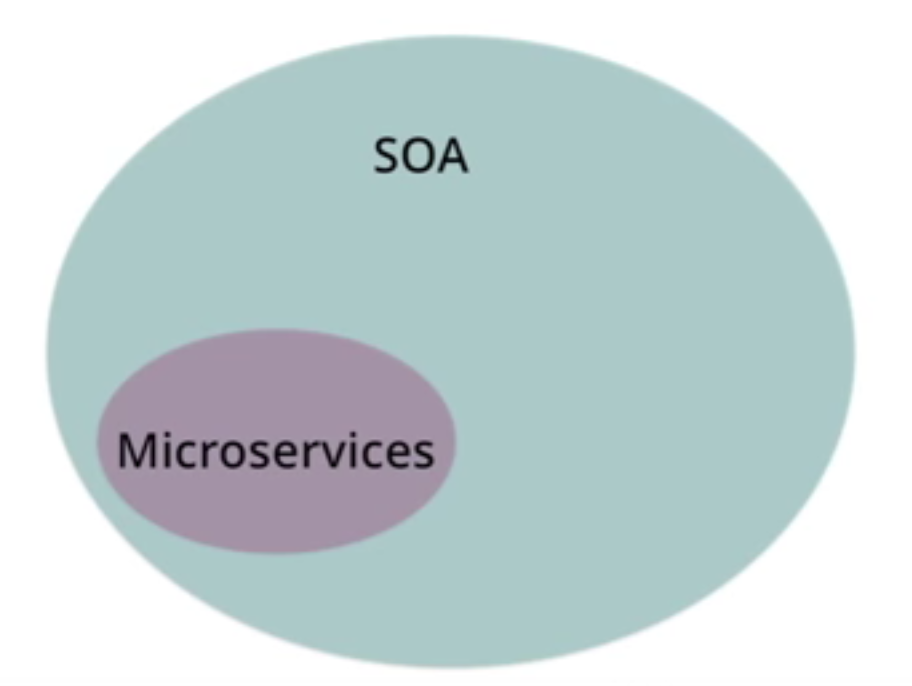
\includegraphics[scale=1]{soavsmicro.png}
\end{figure}

\subsection{Internal integration}
Typically when a new component has to be added to an existing
project the approach consists in the development of a library which
has the logic to deal with the new module to be supported. Subsequently the component
will
become part of the project itself, with its needs to be updated throughout time.
However when the number of components to integrate increases it will affect the size
of the project and very likely its performances.
In our case the component to be integrated will be the ecosystem driver,
having a set of libraries which are capable of interacting with the remote APIs or
with the direct wired connections. As we'll see in the next paragraph this is a typical
monolith approach, meanwhile for this situation would be better to use a microservice approach.

\subsection{Integration as a Service}
Considering the \textit{Microservice} architectural pattern we can decompose
the above situation creating dedicated services capable of handling the
required business logic to interact with an external system. This approach
is also called \textbf{Componentization via Services}[7], where a component is defined
as a \textit{unit of software that is independently replaceable and upgradeable.}
It is important to distinguish between \textit{libraries} and \textit{services}:
the latter uses out-of-service components to communicate, mainly HTTP requests or
remote procedure calls when libraries uses instead mechanisms like in-memory calls.
The main advantage to build components as services instead of libraries is the
possibility to deploy them individually without the need to redeploy the whole system.
If a library is modified or removed the whole system will need to be redeployed,
which in most of the cases it is converted in a loss of money and time. That's not
the case if the system is composed by many independent systems, where only the changed
service will need a new deployment. However this is not always true, there will be some
circumstances where it will be necessary anyway to deploy again the whole system, but the
aim of this approach is to reduce the number of these necessities.

\subsection{Other benefits}
Apart from the benefits already listed formerly, there are other benefits introduced by
adopting the microservice architecture:

\begin{description}
  \item[Heterogeneity between technologies] Structuring the system as a set
  of services frees us from the limitations of a singular technology allowing
  us to adopt different frameworks for different tasks. This benefits on the
  possible optimization that can be achieved using the right technology for the
  right task. Furthermore this removes completely the problem of creating adapters
  for different technologies to integrate in the system if they do not exist. This is
  also called \textbf{Decentralized Governance}.
  \item[Evolutionary Design] is a concept popularized by the \textit{Extreme Programming},
  where the system is continuously evolving during the phases of it's development.
  This key feature makes possible to evolve adopting a microservice architecture while
  keeping the old legacy monolith system, well tested and functional, without rewriting
  the whole system.
  \item[Designed for failure] Building a system made of services instead of components
  leads the developers to take more effort in considering failures. Developers have
  to take in consideration the possible failure while reaching the service, and
  prevent the system to crash and handle the situation in the most gentle way. On the
  other side, this approach introduces more overhead to handle the possible situations.


\end{description}


\subsection{Microservice Oriented Internet of Things}
IoT with their advent brought up some, not yet resolved, challenges which fits
very well with the Microservice architecture. \textit{Interoperability} is one of these
challenges aimed to be solved. Microservices \textit{decentralized governance} feature,
which allows the use of different technologies inside the same systems holds the key for
solving the interoperability problem. Key IoT devices vendors realizes that if their products
supports multiple interoperability standard they're likely to be adopted also by their
competitors (e.g. Nest products are available on HomeKit).[3] Microservices here can be
used as isolated adapters for the many different technologies, facing the spreading
fragmentation of communication protocols between machines.\\
Microservices are by nature dynamic and reactive, which makes them a good choice for
an environment where new technologies are frequently added or modified.

\section{Calvin}
  \textit{Calvin} is an Open-Source distributed framework designed mainly, but not only,
  for IoT systems. The key point of \textit{Calvin} is the "Distributed cloud for IoT", meaning
  running the code where it best suits the performance needs, a crucial aspect since we are
  dealing with low-resource components. We will use \textit{Calvin} for the whole course of the document,
  referring to it as the main "system", also used to integrate with the others. \\
  \textit{Calvin} has the ability to integrate new components without replacing them by writing
  proxies for the specific hardware to support. Proxies are actors written to handle
  communication with the legacy system. Such a proxy actor handles the task of converting data
  from the application into messages or requests the old system can handle, and converting the
  response back into tokens the Calvin application understands.[14]

        \begin{figure}[h]
        \caption{Proxies interaction}
        \label{fig:calvinproxy}
        \centering
        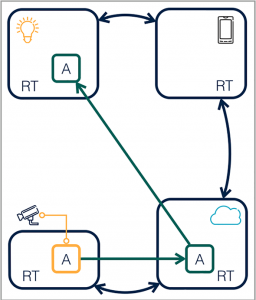
\includegraphics[scale=0.75]{calvin4.png}
        \end{figure}
  Figure \ref{fig:calvinproxy} shows the interaction of native Actors and Actors which
  acts as a proxy for legacy components, in this example the camera.




  \textit{Calvin} is built upon the well-established actor model, using a methodology often referred to as dataflow programming[11], and
  its life cycle can be summarized in four, well-distinct, phases: \textit{Describe}, \textit{Connect}, \textit{Manage}
  and \textit{Deploy}.

\subsection{Describe}
  The smallest functional units in \textit{Calvin} is an Actor. Actors do not share
  nor state or behavior, encapsulating all the logic. The key point of Actors in Calvin
  is their reactivity: they react to external events or when receiving inputs. Actors
  communicates only using data through ports, has to be defined before deploying the system.
  This way is possible to describe the possible interactions that the actor may have when
  connecting it to others.\\
  Having a non-shared internal state allow the Actor to be serialized and moved to another
  running machine or to be backed up if the machine crashes. However this is partly true because
  it may be tricky to serialize Actors with a very complex internal state.

  \begin{figure}[h]
  \caption{Describe Phase}
  \centering
  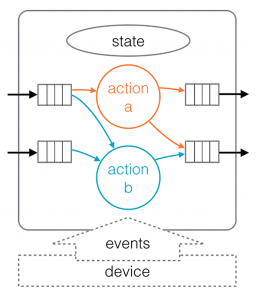
\includegraphics[scale=0.75]{calvin1.png}
  \end{figure}


\subsection{Connect}

    \begin{figure}[h]
    \caption{CalvinScript Example}
    \label{fig:calvinscript}
    \centering
    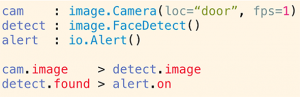
\includegraphics[scale=0.75]{calvin2.png}
    \end{figure}

  After describing the many functionalities provided by the various Actors in the system
  we need to tie them to build applications. \textit{Calvin} offer a scripting language,
  named \textbf{CalvinScript}, to describe the various connections between actors
  and their input and output ports. In figure \ref{fig:calvinscript} there is an example
  of a script for detecting faces in an image. The first part is relative to the actors declaration
  and initialization, giving a clear description of which actors will be playing in the current
  environment. The second part describes the links between each actors, structuring the flow
  of the process. In this case the actors in the system are 3: the \textit{Camera}, the \textit{Detector}
  and the \textit{Alert}. The flow of the process is relatively simple in this case, and it is structured
  as follows: the  \textit{Camera} takes a picture, which will be passed to the \textit{Detector}. Subsequently
  the \textit{Detector} will send its result to the \textit{Alert} actor, which will possibly fire an "alarm" if he
  detects any human face inside the picture.\\
  Figure \ref{fig:calvinactors} shows a more complex interaction between actors. %%[TODO] maybe add something here about the picture

  \begin{figure}[h]
  \caption{Actors interaction}
  \label{fig:calvinactors}
  \centering
  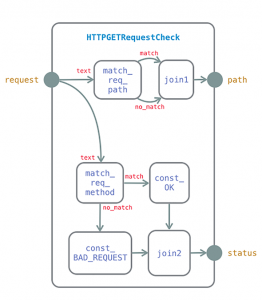
\includegraphics[scale=0.75]{calvin3.png}
  \end{figure}



\subsection{Deploy}

  Each Actor has different resource requirements needs to be satisfied in order to be
  deployed successfully. For example, referring to the previous scenario, an actor
  using a camera needs to be deployed on a system where there actually is a camera. These
  are also called \textit{hard} or \textit{unconditional requirements}, which determines
  the possibility to instantiate or migrate the actor on a machine. \\
  On the other side there are also \textit{non-functional requirements}, describing where
  an actor would suit best for its task. Always referring to the former example, when applying
  face detection it would be better to perform this task on a more performing machine compared to
  a low-resource machine, like a \textit{Raspberry Pi}.\\
  However at the moment \textit{Calvin} supports only \textit{static deployment}, needing the user
  to define where to deploy and execute the actors.

\subsection{Manage}
  When the whole runtime is running it is more than needed to have a tool to keep
  track and monitor the activities in the system. The runtime can be queried to retrieve
  informations about the actors and locate them. It is also possible to track
  the actors firings, on which ports and step by step execution. These are mainly
  debugging tools, though it is also true that this is a recent framework and many
  functionalities are already in development.


\subsection{The relationship between the Actor Model and Microservices}
Actors are isolated, single-threaded components that encapsulates both state and behavior.
Typically actors communicates using lightweight direct messaging systems, for example
to receive or return inputs/parameters. Microservices are very similar to Actors in many
of their key aspects, such as isolation, encapsulation and lightweight messaging, though
usually microservices uses RESTful interfaces. There is some discussion
in the community whether some argues that actors are actually microservices
themselves [12] meanwhile others defines actors as a subset of microservices[13].
This however heavily depends on the actors framework adopted for the situation, which in our
case an Actor can not be compared to a microservice due to an insight limitation: \textbf{Calvin Actors can not
use different technologies}, at the moment.

\subsection{Calvin's Three Tier architecture}

Calvin is structured with a three tier architecture: the actor layer, the system layer and the runtime layer.
Each of them is isolated and can communicate with each other only passing values through the various
layers. The architecture is summarized in picture \ref{fig:calvinlayers}

\begin{description}
    \item[Actor Layer] The actor layer is the upper layer which exposes all the actors and their functionalities.
    Actors can used only the functionalities offered by the lower level calvinsys with no direct access to the runtime
    system.
    \item[Calvinsys Layer] Calvinsys is considered the middleware, where all the runtime logic is exposed through
    high level functions and objects. This layers wraps and uses the functionalities offered by the runtime layer,
    offering tools for the development of advanced actors.
    \item[Runtime Layer] the runtime layer is considered the core, in this layer are stored all the low level
    implementation.In this layer can be found detailed implementations of how to communicate with different kinds
    of sensors, an asynchronous implementation of HTTP calls for Calvin and etc. Here's the core of all
    the functionalities adopted by the higher level objects such Actors or middleware libraries.
\end{description}

\begin{figure}[h]
\caption{Calvin Architecture}
\label{fig:calvinlayers}
\centering
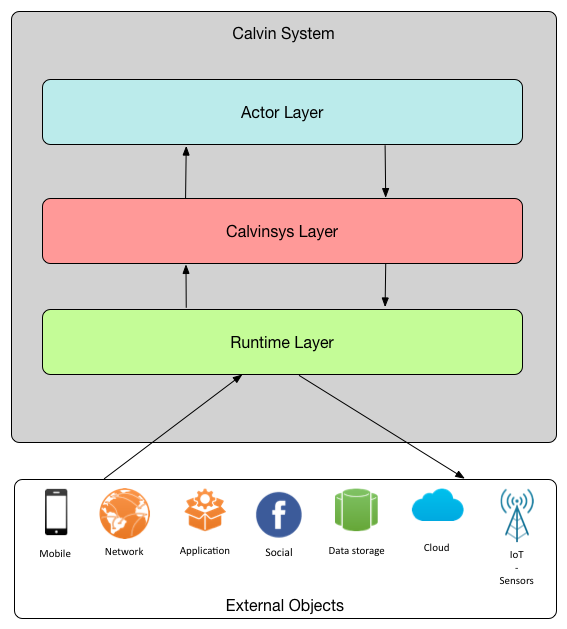
\includegraphics[scale=0.45]{calvinlayers.png}
\end{figure}


\subsection{Anatomy of an Actor}

As previously introduced Actors are abstract reactive entities which exposes inbound and outbound connections.
In contemplation of \textit{reactivity} all the actions taken from an actor must be simple, fast and short. Nonetheless
this optimal situation is hardly achievable in real life, it's usually more common to have blocking calls to services
in the runtime which require on average more then 1-2 seconds. This limitation can be solved simply moving the logic
in the runtime towards an asynchronous approach for long time tasks. Typical tasks requiring asynchronous interaction
can be reading data from a sensor, sending an HTTP request or authenticating into any service, the list is longer but
can summarize in most of interaction with out of the system objects.\newline
An actor anatomy can summarized in the following parts:
\begin{itemize}
    \item Declaration of the connections
    \item Initialization and setup
    \item Migration
    \item Actions, Guards and Conditions

\end{itemize}

\subsubsection{Declaring the connections}

All the connections of an actor has to be declared a priori, and hence be all used (or allocated)
when the actor is used. The declaration is done simply adding under a comment the names of the many connections
and their type: either input/output or both. Here is a simple example of an actor for HTTP GET requests:

\begin{verbatim}
    Input:
      URL : URL to get
      params : Optional parameters to request as a JSON dictionary
      header: JSON dictionary with headers to include in request
    Output:
      status: 200/404/...
      header: JSON dictionary of incoming headers
      data : body of request
\end{verbatim}

In this example we can see the 3 input ports: URL, params and header, which will all be needed to be set
in order to fire one of the actions, depending on the condition. These inputs can be used
as a condition parameter using \texttt{action\_input['var\_name']} and \texttt{action\_output['var\_name']}
for outputs.\\
However it is very likely that we won't need all these inputs or outputs, specially if they are optional
like \texttt{params}. For this reason there exists two special actors which will connect to these
ports without generating tokens or consuming them without doing anything (namely Void and Terminator).

\subsubsection{Initial phase}

The initial phase is denoted by the decorator \texttt{@manage['inputs']}, where all the variables
are set and the required libraries are loaded. It is possible to pass inputs at instantiation
time using manage and bypassing the input ports, though this approach is discouraged and
advised only for particular situations. Furthermore in this phase all the components
from the \textit{calvinsys} will be loaded for a consequent use during the actor actions.

\subsubsection{Migration}

One of \textit{Calvin's} key feature is the simplicity of migrating actors through the
different nodes in a cloud system. Migration of the object is achieved using a special function
\texttt{migrate(self):} to which can be passed the current actor object, and it will be serialized.
Migrating implies serializing all the current variables which composes the actor's state to be sent, though
problems may arise if these variable contains complex objects such as connections (e.g. DataBase connection,
TCP connection etc). When the state will be sent to another machine, this will setup the actor
passing from the former phase, hence creating a new (almost) identical actor.

\subsubsection{Actions, Guards and Conditions}

The core of an actor are the actions it can perform, but these needs some conditions to bet met
before being fired (e.g. having a variable set to \texttt{true}). Most of actions are composed of three
key elements:

\begin{description}
    \item[Condition] is a mandatory decorator which describes the inbound and outbound connections for the action.
    Although the name suggests it to be the condition statement to for firing an action, condition is related to the
    input and output condition of the action. An example of condition for a camera actor can be
    \texttt{@condition(action\_input=['trigger'], action\_output=['image'])}. In this case our actor when will receive a token
    on the \texttt{trigger} port will enable the action, but the next decorator will be the definitive check to pass to the action
    body.
    \item[Guard]  is an optional decorator, for checking some conditions before passing to the body of the action.
    Guard is more related to the internal state of the actor instead of the connected ports, thus it's the real condition
    check to fire the action. Guard can be used to see if a variable has been set or if its value is correct. For example
    if we want to check that an actor has completed an asynchronous task we can use a guard similar to this one:
    \texttt{@guard(lambda self: self.camera.picture\_taken)}. In this case \textit{Calvin} will perform an evaluation
    of one the actor internal objects: it the value is set to \texttt{true}, it means that the picture has been taken and
    its stream has been saved on the disk (i.e. the file exists). This allow the system to prevent firing actions
    when the actor may not be ready for it even though the firing connections are set.
    \item[Action] The action is a simple function which has to take as parameter the inbound values in the condition
    statement, and return an \texttt{ActionResult} object with the expected output bounded to the outbound values.

\end{description}

Moreover inside the actor the actions has to be listed by priority, to avoid ambiguity
when choosing with the correct action to fire. 

\chapter{Detecting Intruders}


\section{Preface}
The major problem faced during this work is related
to the detection of intruders while surveilling the house.
Modern security systems applies different techniques to detect intrusions
using many different sensors such as leap motion detection, face detection
or sound analysis. They have been working fine during the last years, however
thieves improves bypassing or partially avoiding these technique making the latter
less effective.\\
Therefore most of the work will be done investigating and testing innovative and
advanced techniques to deal with intrusions detection.

\section{Fingerprinting a Human}

During the time there has been many approaches to recognize a "Person"
using some of its peculiarities: software side with passwords or access phrases,
which should identify a single person; biometrics with finger prints, retina scans
and voice recognition.\\
Usually such controls where available only with expensive solutions (and some still are, e.g. retina
scanners), however with the introduction of \textit{IoT} their price dropped allowing
them to be sold for a reasonable price. These controls are also called \textbf{behavioral biometrics},
the set of behavioral traits which identifies an individual person. Usually these traits are
used for authentication when accessing a restricted system, however we'll consider
these to recognize unknown entities accessing our house. \\
These systems are mainly needed to prevent accidental triggering of the alarm, to be more
precise when listening or watching, not detecting just something but a real intrusion.

\subsection{Behavioral biometrics}
Detecting if someone in the house is someone familiar is not an easy task, most
of the approaches are precise in optimal conditions, much less when the situation
is non optimal (low light, low resolution etc). This impacts negatively their efficiency
when applied in a real life scenario, where usually the conditions are far from the optimal
situation. For example facial recognition works in very limited cases, like the systems
used on smartphones to unlock the device, has been reported to not be reliable enough
to be the main unlocking system. The situation is also similar for voice recognition or
speech to text systems, which are improving during the time and mainly \textbf{during the usage}.
\textit{Siri}, one of the most famous personal assistant had some minor troubles at the beginning
being used to the different users voices, accents and languages. \textit{Siri} uses
different voice recognition algorithms to categorize your voice by learning your
dictation and your accent, with good results over time.



\section{Expanding the system}
One of the biggest limitations of nowadays security system is their isolation
when installed. Most of devices are stand alone solutions incapable of extending
their functionalities to pre existing devices. If we want to expand \textit{Calvin} to
be adopted by others, including users and developers, we need to be able to extend its
functionalities with the ability to communicate with different other systems.

\section{The Architecture}

In this section we will go deep in the details of the architecture of the solutions
we propose.

\subsection{Accessing different systems}

Accessing different systems is a problem of technology interoperability between
different technologies running on architecturally different hardwares.
Most of the times \textit{IoT} devices runs on low limited power devices such as
an \textit{Arduino} or a \textit{Raspberry Pi}, both supporting different system
languages (the first is limited to a subset of \textit{C++} meanwhile the second one supports everything
that can run under a normal linux distribution, but usually it's \textit{Python}).
However in our scenario the devices we consider are on a different layer of abstraction,
we do target ecosystems and not single independent devices. \textbf{Ecosystems} has to
provide an access to developers through a point of access, \textbf{REST api} for   \textit{Nest}
and the \textbf{HomeKit.framework} for accessing \textit{HomeKit} devices.
The limitations are not always the same, when using \textit{Nest} it's easier to communicate
with it using a wrapper for their own api, which exists in many libraries, including \textit{Python}.
Nonetheless the situation with \textit{HomeKit} is much more strict, having their ecosystem
restricted only to their technology, \textit{Objective-C} or \textit{Swift}, which runs only
on \textit{Apple} branded device. Furthermore, the limitations are even more strict
due to the limitation of the framework only for \textit{iOS}, at the moment at least.
Usually the latter is the common case, which implies the need of a different solution
then "just wrapping" the apis in the code and plug them into the project.
In our case \textit{Calvin's} system is fully written in \textit{Python},
though it have many extension for a wide range of technologies, communicating
with \textit{HomeKit} is still hard to achieve.
In the following sections we'll describe the approaches taken to solve
the problem.




\section{Accessing Nest}

As said in the previous section \textit{Nest} has some advantages
due to their cloud apis, which makes it easier to reach the connected devices.

\subsection{Nest API Model}

\textit{Nest} offers a cloud API near real time, based on a subscription, that allows
users to build products accessing data on their devices, with the relative ability
to read and write data. With the \textit{Nest} cloud each element is identified as a resource
and accessible through a unique address, called "data location".
Furthermore, the cloud system also offers a \textit{RESTful} service to access these resources,
but only allowing GET and PUT operations with a call limit to prevent overuse. There is also
a \textbf{Streaming} feature for REST, which allows our application to receive updates
in real-time or to stream from a device, namely camera, since web-sockets are not supported.
However it applies the same rule as before, with some limits in the data usage to prevent abuse.

%%[TODO] maybe add some more description or api usage examples

However, the cloud functions of \textit{Nest} are limited to a restricted set of devices:
Thermostat, Protect (alarm), Camera and the Home.
Here are the functionalities offered by each of the products, with a brief description:
\begin{figure}[h]
\caption{Nest Cloud architecture}
\label{fig:nestarch}
\centering
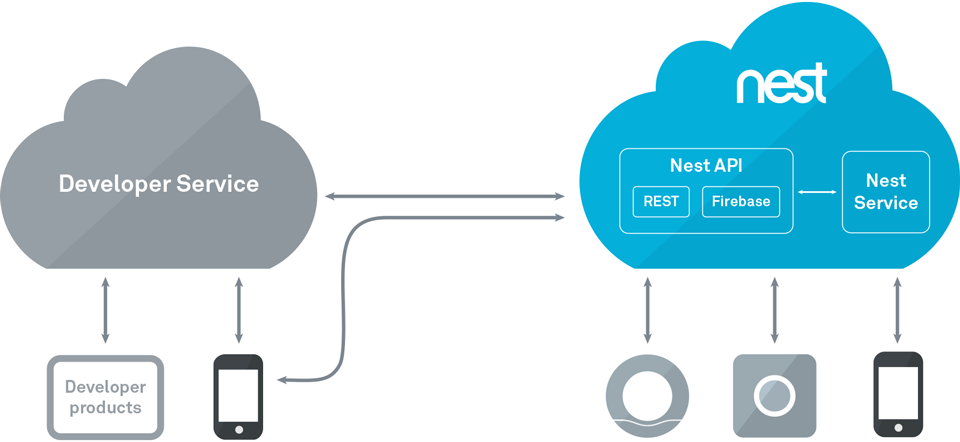
\includegraphics[scale=0.35]{nest-architecture.png}
\end{figure}

\subsubsection{Nest Thermostat}
Thermostat, as the name suggests, is a smart thermostat ,which can also be remotely controlled,
with some energy saving settings to help the user avoiding unnecessary heating expenses.   \\
Its remote functionalities are:

\begin{itemize}
    \item Read the current temperature
    \item Read or set a target temperature
    \item Set the fan timer
    \item Read or set the temperature mode
    \item See humidity values
    \item View online status and last connection information
    \item Read structure name and device location in the home
\end{itemize}

\subsubsection{Nest Protect}
Protect is a location based alarm for dangerous gas leaks, such as  Carbon monoxide \textit{CO}, or
smoke in case of fire.

\begin{itemize}
    \item View CO or smoke status
    \item View battery health state
    \item View last manual test status and timestamp for last manual test
    \item View online status and last connection information
    \item Structure name and device location in the home
\end{itemize}

\subsubsection{Nest Camera}
Camera, previously known as Dropcamera, is one of they key components of the
\textit{Nest} suite. It provides screen capture, audio and video streaming and the
other typical features offered by smart cameras.

\begin{itemize}
    \item View camera online status or mic status
    \item View or change streaming status (turn video streaming on/off)
    \item View device name and where identifier
    \item View last online status change (last online/offline change)
    \item View subscription status (enrolled/not enrolled)
    \item Learn more about Nest Aware with Video History subscriptions >
    \item View deep links to the live camera feed in the Nest app (iOS, Android) or on the web at home.nest.com
    \item View content related to the last event that triggered a notification, including:
        \\Sound or motion event detected
        \\Event start/stop times
    \item Deep links to image and gif files
    \item Structure name and device location in the home

\end{itemize}



\subsection{Nest with Calvin}

%%[TODO] create a nice chart to describe this
One of the key aspects of \textit{Calvin's} Actors is their abstraction
to allow their reuse in different situations. However, due to the different
nature of the ecosystem, specially \textit{Nest} and \textit{HomeKit} the actors
can't be used for the same purpose.
\textit{Nest} structure can be decomposed in two big sections: Structures and Devices.
Structure are objects to keep grouped together many devices, placing them in different part of the house,
but still not the most important part in our scenario.\\
A device is an abstraction of all the smart products offered by Nest, but mainly the one we have listed in the latter
paragraph.

\subsubsection{Device Abstraction}

We have abstracted a device in its most basic functions: setting and getting properties.
This simplification allows us to follow the best practices for the development of \textit{Calvin},
allowing a possible reuse of the actor. Here is the pseudocode for the high-level functions definition.

\begin{verbatim}
    getproperty: in device_id, property_name; out property_value
    setproperty: in device_id, property_name, value ; out True or False
\end{verbatim}


However going deeper into the actor architecture we have to define some more constraints,
like the events which trigger the execution and the tokens for which returning the results.
First of all, all incoming port of an actor has to be linked, we can not have an unbounded port,
both input or output. Here's a list of our actor's ports:\\

\begin{verbatim}
    Inputs:
        device: the device identifier
        operation: string representing the operation to do (get or set)
        property_name: the property to be get/set
        value: the value to be used to set the property
    Outputs:
        result: the property value
\end{verbatim}

To simplify the work, we reduced the inbound port for the operation to only one, instead of having a token
for a \textit{get} or \textit{set} operation. This task is completed using the \texttt{@condition} to declare
all the elements which are needed to fire and will be used in a particular action.
A simple condition for an action is the following example:
\begin{verbatim}
    @condition(action_input=['operation'], action_output=[])
\end{verbatim}
This condition requires the token operation to be bounded, and it will use it in its body function. Since
no \texttt{action\_output} is defined, the operation does not return any value.

Once all the inbound ports are connected, i.e. they have a token, the system will check the \texttt{@guard} condition,
which acts as a conditional control: it will continue only if the condition is satisfied.
An example guard condition can be written as:

\begin{verbatim}
    @guard(lambda self: self.nest._in_progress is None and self.operation == "set")
\end{verbatim}
This guard condition is used to enter the function only when the \textit{nest} object is not
working on an asynchronous task and the operation has to be the \textit{set} operation.\\
One of the constraints that an actor has to follow is the \textbf{reactivity}, which implies
non-blocking calls in the body of its functions. However, as in our case, the actor will have to
make some calls to the \textit{Nest} cloud, which is a blocking call. This is reached
using a two step asynchronous system: first the value is acquired and the actor
will delegate the request to a different thread; second when the delegate terminates it will
modify a flag to mark its completion, at that point the actor will return the value obtained
from the nest cloud. Asynchronous calls are needed since the scheduler loop can't be blocked
during the execution otherwise it would break the reactivity of the other actors.

\subsection{A Microservice Oriented approach}

Despite of the correctness of the former solution, it does however contains some
flaws in the architecture. The solution works with under the following circumstances:

\begin{enumerate}
    \item Libraries for connecting to a different ecosystem are provided in the same language (e.g. \textit{Python}).
    \item We assume the actor does never crash, and if it does the system may crash subsequently.
    \item The integration library won't require any change or modification in the future.
\end{enumerate}

However these assumptions are too risky to be considered for an always running system, because the likeliness
of one of the above problems to happen is very high.\\
To face these problems we adopted a \textbf{microservice} architecture style to implement the integration with
other ecosystems. In the case of \textit{Nest} is not very significative but it will be much more for \textit{HomeKit}, as
we'll see later.

\subsubsection{Microservice Architecture}


\begin{figure}[h]
\caption{Microservice Integration architecture}
\label{fig:test-arch}
\centering
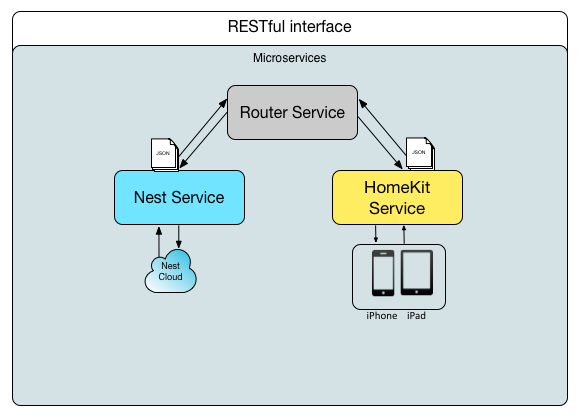
\includegraphics[scale=0.65]{test-arch.png}
\end{figure}

Figure \ref{fig:test-arch} illustrates the architecture proposed in our solution.
All the microservices can be reached through a router service, which doesn't expose
the real location of each service. This approach moves the service finding logic outside
of \textit{Calvin}, simplifying the work of the actor who won't have to deal with possible
re-deployments or re-locations of the service, it will just need to know where to reach the
routing service. This task will be deferred to the \textit{routing} service, which will act
as a proxy to the other micro-services.\\
Each ecosystem has a microservice dedicated, this is due to the different internal structure of the
different technologies. For example \textit{HomeKit} uses a hierarchical structure divided in the following,
from above to the bottom: \textbf{HMHome}, \textbf{HMRoom}, \textbf{HMAccessory}, \textbf{HMService} and \textbf{HMCharacteristic}.
Which differs from the simpler one of \textit{Nest}, where there are mostly Structures and Devices.\\
Moreover structuring the integration with ecosystems introduces the capability to link more accounts, more devices,
to the \textit{Calvin} runtime.

\subsubsection{The microservice API}

The API to describe the connection between \textit{Nest} and the microservice
resembles the former actor structure.
Following the classic \textit{RESTful} style, to access a device will look like
\begin{verbatim}
    Url
    GET /device/<deviceid>

    Example Response
    {"device":
        {
        "name": "DFF9", "temperature": 37, "humidity": 50, "fan": false,
        "mode": "heat", "online": false, "serial": "fake9396122EDFF9",
        "where": "basement","structure": "HomeTest", "target": 25
        }
    }

    [TODO] add all the other calls
\end{verbatim}





\subsection{Accessing HomeKit}

\textit{HomeKit}, introduced in details in the previous chapter, is the other ecosystem
for which we are extending \textit{Calvin} integration. First of all, HomeKit doesn't
expose any cloud API, it's functionalities can be accessed only through their \textbf{HomeKit.framework},
a library available only for \textit{iOS}. As can be seen the limitations compared to Nest
are much more strict, which implies no direct integration. The only possible solution for the
moment is to have an \textit{HTTP} web server exposing HomeKit functionalities to the outside of
the world. As previously mentioned, their library is not available on both \textbf{Mac OS X} nor
the Apple TV \textbf{tvOS}, which means the only possible approach is a mobile application.
However it is predicted to be supported by the former OS in the future, on which would be a more
elegant and nicer solution.\\

\subsubsection{Understanding}















\subsection{lol}
The answer is 42

\appendix
\chapter{Tables}

\begin{table}
\caption{Armadillos}
\label{arm:table}
\begin{center}
\begin{tabular}{||l|l||}\hline
Armadillos & are \\\hline
our	   & friends \\\hline
\end{tabular}
\end{center}
\end{table}

\clearpage
\newpage

\chapter{Appendix - Figures}


\begin{figure}[h]
\caption{Model audio specter}
\label{fig:specter}
\centering
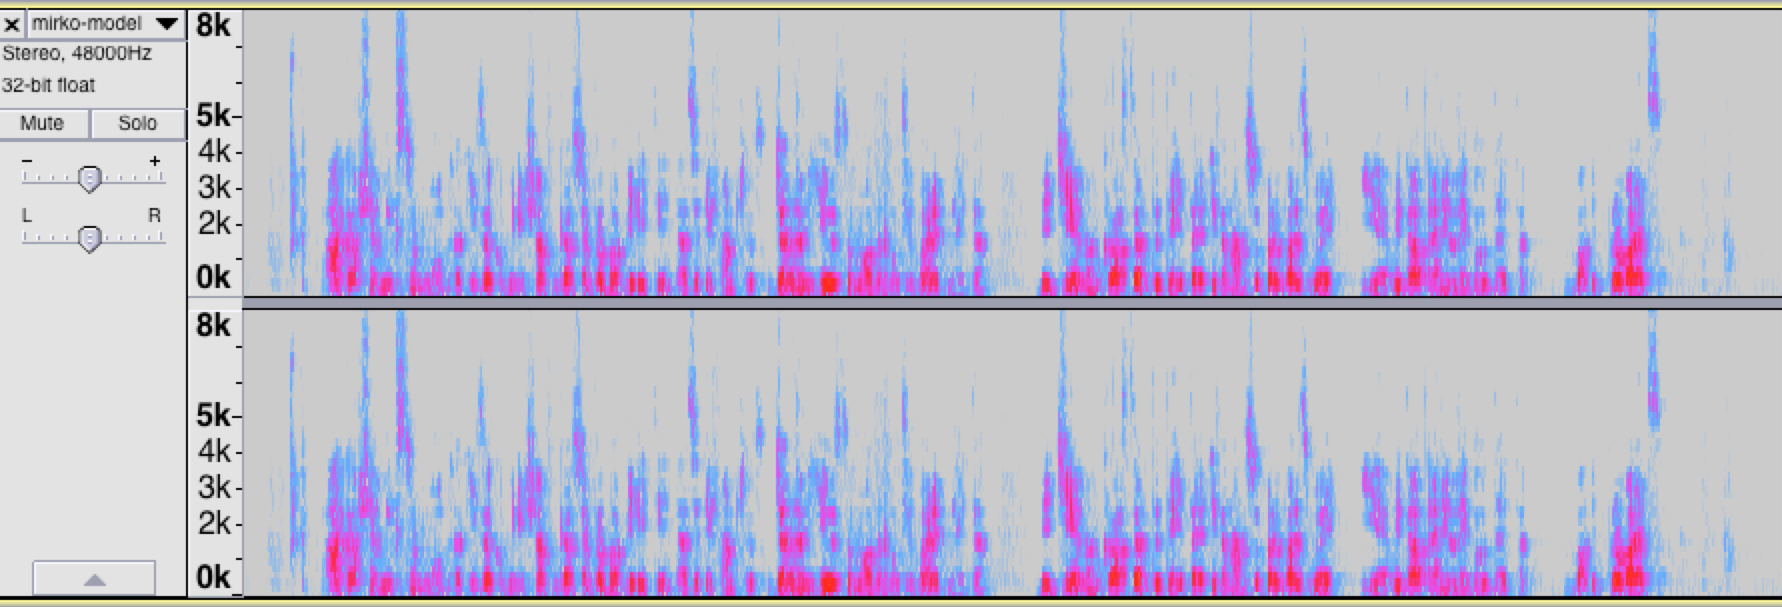
\includegraphics[scale=0.23]{model-spectre.png}
\end{figure}
\begin{figure}[h]
\caption{Model audio wave}
\label{fig:wave}
\centering
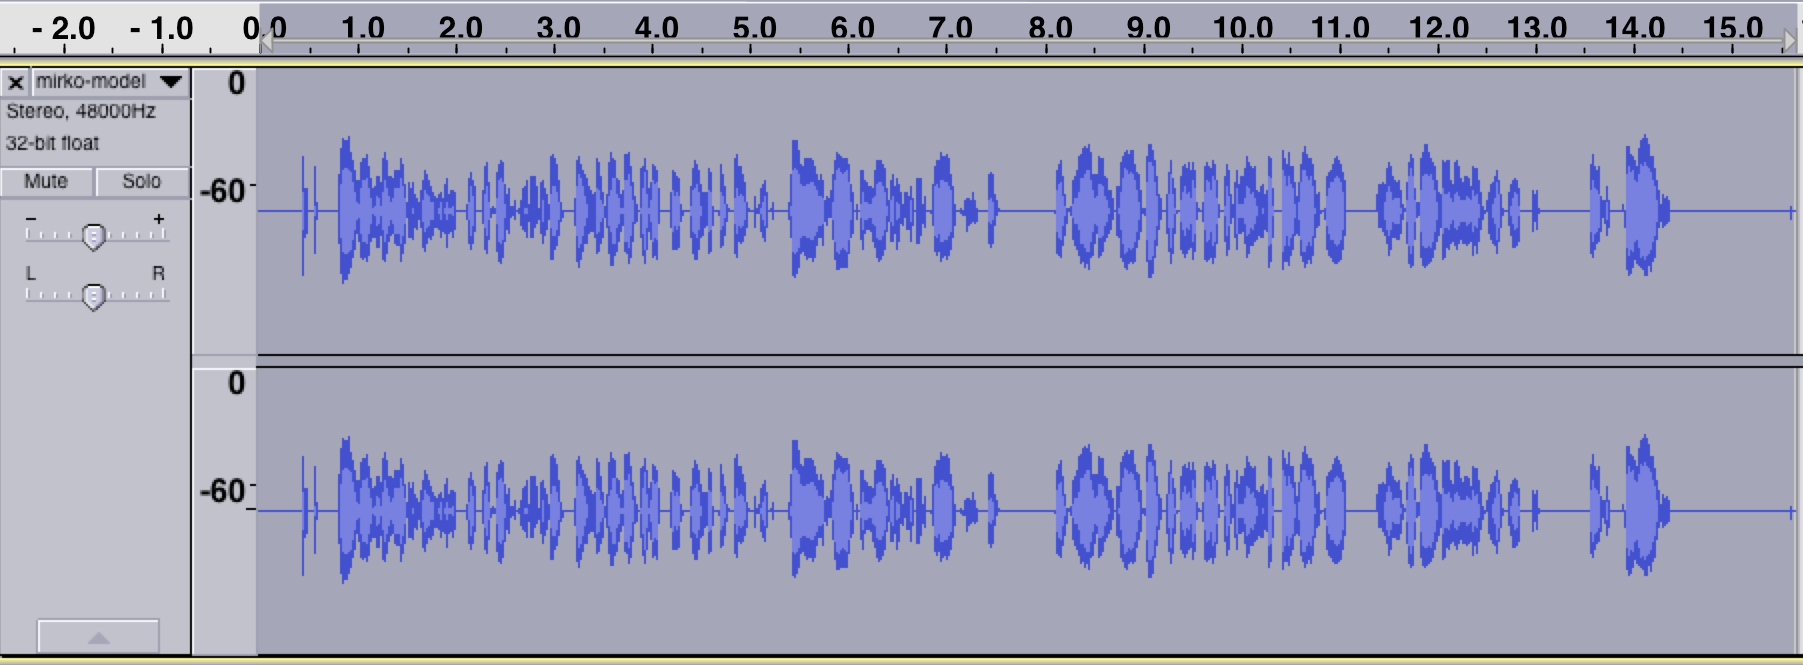
\includegraphics[scale=0.23]{model-wave.png}
\end{figure}

%% This defines the bibliography file (main.bib) and the bibliography style.
%% If you want to create a bibliography file by hand, change the contents of
%% this file to a `thebibliography' environment.  For more information 
%% see section 4.3 of the LaTeX manual.
\begin{singlespace}
\bibliography{main}
\bibliographystyle{plain}
\end{singlespace}

\end{document}
